\documentclass[man]{apa6}
\usepackage{lmodern}
\usepackage{amssymb,amsmath}
\usepackage{ifxetex,ifluatex}
\usepackage{fixltx2e} % provides \textsubscript
\ifnum 0\ifxetex 1\fi\ifluatex 1\fi=0 % if pdftex
  \usepackage[T1]{fontenc}
  \usepackage[utf8]{inputenc}
\else % if luatex or xelatex
  \ifxetex
    \usepackage{mathspec}
  \else
    \usepackage{fontspec}
  \fi
  \defaultfontfeatures{Ligatures=TeX,Scale=MatchLowercase}
\fi
% use upquote if available, for straight quotes in verbatim environments
\IfFileExists{upquote.sty}{\usepackage{upquote}}{}
% use microtype if available
\IfFileExists{microtype.sty}{%
\usepackage{microtype}
\UseMicrotypeSet[protrusion]{basicmath} % disable protrusion for tt fonts
}{}
\usepackage{hyperref}
\hypersetup{unicode=true,
            pdftitle={Sensitivity analysis for the robustness of effects in psychological science},
            pdfauthor={Joshua Rosenberg~\& Ernst-August Doelle},
            pdfkeywords={keywords},
            pdfborder={0 0 0},
            breaklinks=true}
\urlstyle{same}  % don't use monospace font for urls
\usepackage{graphicx,grffile}
\makeatletter
\def\maxwidth{\ifdim\Gin@nat@width>\linewidth\linewidth\else\Gin@nat@width\fi}
\def\maxheight{\ifdim\Gin@nat@height>\textheight\textheight\else\Gin@nat@height\fi}
\makeatother
% Scale images if necessary, so that they will not overflow the page
% margins by default, and it is still possible to overwrite the defaults
% using explicit options in \includegraphics[width, height, ...]{}
\setkeys{Gin}{width=\maxwidth,height=\maxheight,keepaspectratio}
\IfFileExists{parskip.sty}{%
\usepackage{parskip}
}{% else
\setlength{\parindent}{0pt}
\setlength{\parskip}{6pt plus 2pt minus 1pt}
}
\setlength{\emergencystretch}{3em}  % prevent overfull lines
\providecommand{\tightlist}{%
  \setlength{\itemsep}{0pt}\setlength{\parskip}{0pt}}
\setcounter{secnumdepth}{0}
% Redefines (sub)paragraphs to behave more like sections
\ifx\paragraph\undefined\else
\let\oldparagraph\paragraph
\renewcommand{\paragraph}[1]{\oldparagraph{#1}\mbox{}}
\fi
\ifx\subparagraph\undefined\else
\let\oldsubparagraph\subparagraph
\renewcommand{\subparagraph}[1]{\oldsubparagraph{#1}\mbox{}}
\fi

%%% Use protect on footnotes to avoid problems with footnotes in titles
\let\rmarkdownfootnote\footnote%
\def\footnote{\protect\rmarkdownfootnote}


  \title{Sensitivity analysis for the robustness of effects in psychological
science}
    \author{Joshua Rosenberg\textsuperscript{1}~\& Ernst-August
Doelle\textsuperscript{1,2}}
    \date{}
  
\shorttitle{A tutorial using R and the konfound R package}
\affiliation{
\vspace{0.5cm}
\textsuperscript{1} Wilhelm-Wundt-University\\\textsuperscript{2} Konstanz Business School}
\keywords{keywords\newline\indent Word count: X}
\usepackage{csquotes}
\usepackage{upgreek}
\captionsetup{font=singlespacing,justification=justified}

\usepackage{longtable}
\usepackage{lscape}
\usepackage{multirow}
\usepackage{tabularx}
\usepackage[flushleft]{threeparttable}
\usepackage{threeparttablex}

\newenvironment{lltable}{\begin{landscape}\begin{center}\begin{ThreePartTable}}{\end{ThreePartTable}\end{center}\end{landscape}}

\makeatletter
\newcommand\LastLTentrywidth{1em}
\newlength\longtablewidth
\setlength{\longtablewidth}{1in}
\newcommand{\getlongtablewidth}{\begingroup \ifcsname LT@\roman{LT@tables}\endcsname \global\longtablewidth=0pt \renewcommand{\LT@entry}[2]{\global\advance\longtablewidth by ##2\relax\gdef\LastLTentrywidth{##2}}\@nameuse{LT@\roman{LT@tables}} \fi \endgroup}


\DeclareDelayedFloatFlavor{ThreePartTable}{table}
\DeclareDelayedFloatFlavor{lltable}{table}
\DeclareDelayedFloatFlavor*{longtable}{table}
\makeatletter
\renewcommand{\efloat@iwrite}[1]{\immediate\expandafter\protected@write\csname efloat@post#1\endcsname{}}
\makeatother
\usepackage{lineno}

\linenumbers

\authornote{Add complete departmental affiliations for each
author here. Each new line herein must be indented, like this line.

Enter author note here.

Correspondence concerning this article should be addressed to Joshua
Rosenberg, Postal address. E-mail:
\href{mailto:my@email.com}{\nolinkurl{my@email.com}}}

\abstract{
One or two sentences providing a \textbf{basic introduction} to the
field, comprehensible to a scientist in any discipline.

Two to three sentences of \textbf{more detailed background},
comprehensible to scientists in related disciplines.

One sentence clearly stating the \textbf{general problem} being
addressed by this particular study.

One sentence summarizing the main result (with the words ``\textbf{here
we show}'' or their equivalent).

Two or three sentences explaining what the \textbf{main result} reveals
in direct comparison to what was thought to be the case previously, or
how the main result adds to previous knowledge.

One or two sentences to put the results into a more \textbf{general
context}.

Two or three sentences to provide a \textbf{broader perspective},
readily comprehensible to a scientist in any discipline.


}

\begin{document}
\maketitle

\subsection{Introduction}\label{introduction}

In social science (and educational) research, we often wish to
understand how robust inferences about effects are to unobserved (or
controlled for) covariates, possible problems with measurement, and
other sources of bias. The goal of \texttt{konfound} is to carry out
sensitivity analysis to help analysts to quantify how robust inferences
are to potential sources of bias. This package provides functions based
on developments in sensitivity analysis by Frank and colleagues, which
previously have been implemented in \texttt{Stata} and through an Excel
spreadsheet, in \texttt{R} through the \texttt{konfound} package.

\section{Background on sensitivity
analysis}\label{background-on-sensitivity-analysis}

Often times, inferences about effects are critiqued because of
\emph{biases}, or factors that contribute to an estimated effect being
different from its ground truth value. These biases come from many
sources, such as not including possibly important control variables or
covariates and sample (i.e., selection bias) and measurement-related
(i.e., not measuring the complete nature of a psychological construct)
biases.

Because of the prevalence of this problem, a number of strategies to
address it have emerged. These strategies can broadly be considered as
approach for carrying out sensitivity analysis. These past approaches
have done XXX but YYY. Frank and colleauges (2000, 2004, 2007, 2013)
have extended this past research by doing ZZZ through two frameworks for
approaching sensitivity analysis.

The first approach, termed the replacement of cases approach, uses
Rubin's causal model to interpret how much bias there must be to
invalidate an inference in terms of replacing observed cases with
counterfactual cases. The second quantifies the robustness of causal
inferences in terms of correlations associated with unobserved variables
in a regression framework.

In the remainder of this paper, we first describe these two approaches
in detail. Then, we introduce the \textbf{konfound} package in R, which
provides a unified interface to carrying out sensitivity analysis using
either approach, using either the results from fitted models or values
provided by the user. We show examples from linear and non-linear as
well as mixed effects (or multi-level) models. We also discuss how the
approach can be used to carry out sensitivity analysis for multiple
studies. Finally, we describe a web-based application as an easy
interface for those newer to sensitivity analysis that can serve as a
gateway to more involved uses.

\subsection{Replacement of cases approach to sensitivity
analysis}\label{replacement-of-cases-approach-to-sensitivity-analysis}

This approach to sensitivity analysis focuses upon quantifying how much
of an effect would need to be due to bias to invalidate the inference
about it. In particular, Frank et al. (2013) use Rubin's causal model
{[}cite{]} to characterize how one could invalidate inferences by
replacing observed cases with unobserved cases in which there was no
effect. This framework enables researchers to identify the \emph{switch
point} (Behn \& Vaupel, 1982) whereby the bias is large enough to change
one's belief (one's inferenece) about an effect.

Technically, the approach compares the estimated effect with a given
threshold. The threshold defines the point at which evidence from a
study would make one indifferent to the choices. The threshold is
commonly defined on the basis of statistical significance but can take
other values (i.e., it can be based upon the effect size; Frank et al,
2013). (need some more technical details here; and to provide an
example)

\subsection{Correlation-based approach to sensitivty
analysis}\label{correlation-based-approach-to-sensitivty-analysis}

In many non-experimental studies, there is a concern that a variable not
considered or included in the analysis is related to both the outcome
and predictor of interest. In these cases, not considering the omitted,
confounding variable may mean that estimates are biased--they are
over-confident. In this approach to sensitivity analysis, the strength
of the correlation between a hypothetical omitted variable and the
outcome and predictor of interest is quantified.

(need to edit this and provide an example) Specifically, Frank (2000)
defined the impact of a confounding variable as rx cvr ycv, where rx cv
is the correlation between the unobserved confound and the predictor of
interest and r ycv, is the correlation between the unobserved confound
and the outcome. Frank (2000) shows how to assess how strong the
confounding variable (cv) has to correlate with the predictor (X) as
well as the outcome (Y) to invalidate an inference of an effect of X on
Y.

\section{Tutorial}\label{tutorial}

In this section, we provide a tutorial of the use of \textbf{konfound}
to carry out sensitivity analysis through both the replacement of cases
and correlation-based approach.

First, you can install \texttt{konfound} with the following:

You can then load konfound with the \texttt{library()} function:

\subsection{Example 1: Use of pkonfound() for values from an
already-conducted
analysis}\label{example-1-use-of-pkonfound-for-values-from-an-already-conducted-analysis}

\texttt{pkonfound()} is used when we have values from an
already-conducted analysis (like a regression analysis), such as one in
an already-published study or from an analysis carried out using other
software.

In the case of a regression analysis, values from the analysis would
simply be used as the inputs to the \texttt{pkonfound()} function. For
example, in the use below, we simply enter the values for the estimated
effect (an unstandardardized beta coefficient) (\texttt{2}), its
standard error (\texttt{.4}), the sample size (\texttt{100}), and the
number of covariates (\texttt{3}):

\begin{verbatim}
#> Percent Bias Necessary to Invalidate the Inference:
#> To invalidate an inference, 60.3% of the estimate would have to be due to bias. This is based on a threshold of 0.794 for statistical significance (alpha = 0.05).
#> To invalidate an inference, 60 observations would have to be replaced with cases for which the effect is 0.
#> 
#> Impact Threshold for a Confounding Variable:
#> An omitted variable would have to be correlated at 0.568 with the outcome and at 0.568 with the predictor of interest (conditioning on observed covariates) to invalidate an inference based on a threshold of 0.201 for statistical significance (alpha = 0.05).
#> Correspondingly the impact of an omitted variable (as defined in Frank 2000) must be 0.568 X 0.568 = 0.323 to invalidate an inference.
\end{verbatim}

For this set of values, around 60\% would need to be false due to a
source of bias for the inference to be invalidated (based on statistical
significance and a p-value (or alpha) of .05), possible a very robust
effect. An omitted, confounding variable (sometimes referred to as a
covariate) would need to have an impact (defined as the product of the
confounding variable's correlation with both the predictor of interest
and the outcome) of 0.323, presenting a different interpretation of how
robust this (hypothetical) effect is to a variable which is important
but not included in the analysis.

Here is another example, but one in which the unstandardized beta
coefficient is smaller than its standard error:

\begin{verbatim}
#> Percent Bias Necessary to Invalidate the Inference:
#> To sustain an inference, 89.924% of the estimate would have to be due to bias. This is based on a threshold of 3.97 for statistical significance (alpha = 0.05).
#> To sustain an inference, 90 of the cases with 0 effect would have to be replaced with cases at the threshold of inference.
#> 
#> Impact Threshold for a Confounding Variable:
#> An omitted variable would have to be correlated at 0.387 with the outcome and at 0.387 with the predictor of interest (conditioning on observed covariates) to sustain an inference based on a threshold of 3.97 for statistical significance (alpha = 0.05).
#> Correspondingly the impact of an omitted variable (as defined in Frank 2000) must be 0.387 X 0.387 = 0.15 to sustain an inference.
\end{verbatim}

Note that this use of \texttt{pkonfound()} is equivalent to naming the
arguments, i.e.~for a different set of values:

\begin{verbatim}
#> Percent Bias Necessary to Invalidate the Inference:
#> To invalidate an inference, 41.732% of the estimate would have to be due to bias. This is based on a threshold of -1.282 for statistical significance (alpha = 0.05).
#> To invalidate an inference, 83 observations would have to be replaced with cases for which the effect is 0.
#> 
#> Impact Threshold for a Confounding Variable:
#> An omitted variable would have to be correlated at 0.334 with the outcome and at 0.334 with the predictor of interest (conditioning on observed covariates) to invalidate an inference based on a threshold of -0.14 for statistical significance (alpha = 0.05).
#> Correspondingly the impact of an omitted variable (as defined in Frank 2000) must be 0.334 X 0.334 = 0.112 to invalidate an inference.
\end{verbatim}

We notice that the output includes a message that says we can view other
forms of output by changing the \texttt{to\_return} argument. Here are
the two plots - for the bias necessary to alter an inference
(\texttt{thresh\_plot}) and for the robustness of an inference in terms
of the impact of a confounding variable (\texttt{corr\_plot}) that can
be returned:

\begin{figure}

{\centering 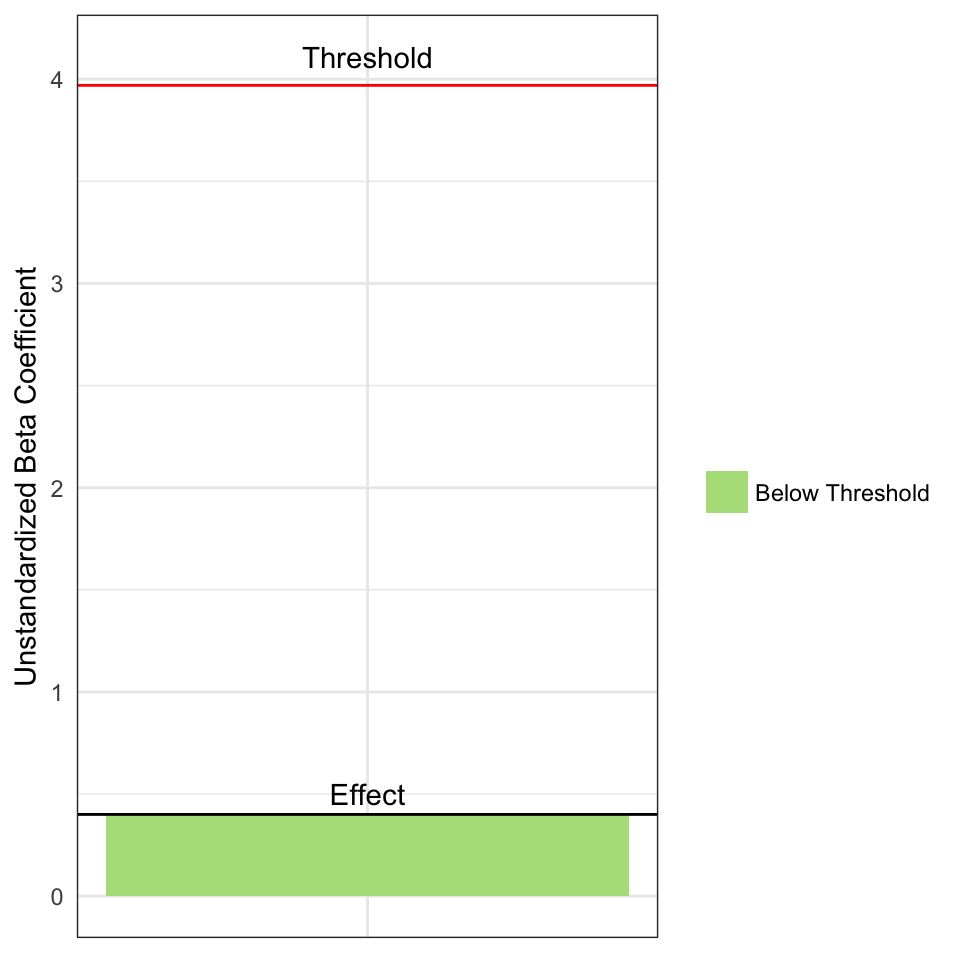
\includegraphics[width=0.7\linewidth]{paper_files/figure-latex/unnamed-chunk-5-1} 

}

\caption{ }\label{fig:unnamed-chunk-5}
\end{figure}

\begin{figure}

{\centering 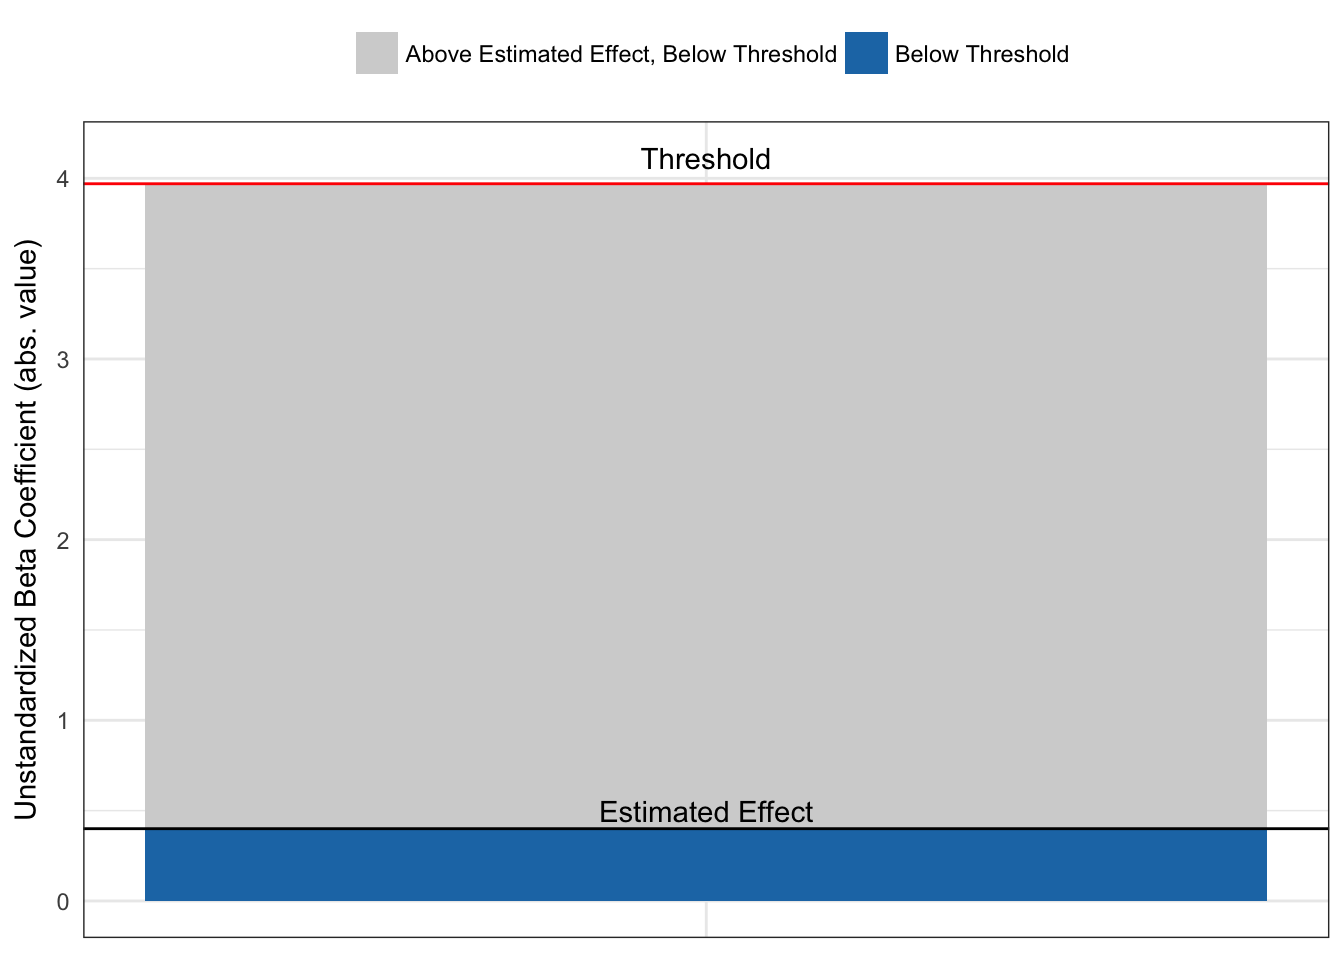
\includegraphics[width=0.7\linewidth]{paper_files/figure-latex/unnamed-chunk-6-1} 

}

\caption{ }\label{fig:unnamed-chunk-6}
\end{figure}

You can also specify multiple forms of output at once.

\begin{verbatim}
#> Percent Bias Necessary to Invalidate the Inference:
#> To invalidate an inference, 60.557% of the estimate would have to be due to bias. This is based on a threshold of 0.789 for statistical significance (alpha = 0.05).
#> To invalidate an inference, 121 observations would have to be replaced with cases for which the effect is 0.
#> 
#> Impact Threshold for a Confounding Variable:
#> An omitted variable would have to be correlated at 0.479 with the outcome and at 0.479 with the predictor of interest (conditioning on observed covariates) to invalidate an inference based on a threshold of 0.14 for statistical significance (alpha = 0.05).
#> Correspondingly the impact of an omitted variable (as defined in Frank 2000) must be 0.479 X 0.479 = 0.229 to invalidate an inference.
#> Created 3 forms of output. To access type: 
#> 
#> model_output$raw_output
#> model_output$thresh_plot
#> model_output$corr_plot
\end{verbatim}

When we type the name of the object, we see that we created three types
of output that we can access as follows:

\begin{verbatim}
#> # A tibble: 1 x 8
#>   action inference percent_bias_to~ replace_null_ca~ unstd_beta
#>   <chr>  <chr>                <dbl>            <dbl>      <dbl>
#> 1 to_in~ reject_n~             60.6              121          2
#> # ... with 3 more variables: beta_threshhold <dbl>,
#> #   omitted_variable_corr <dbl>, itcv <dbl>
\end{verbatim}

\begin{figure}

{\centering 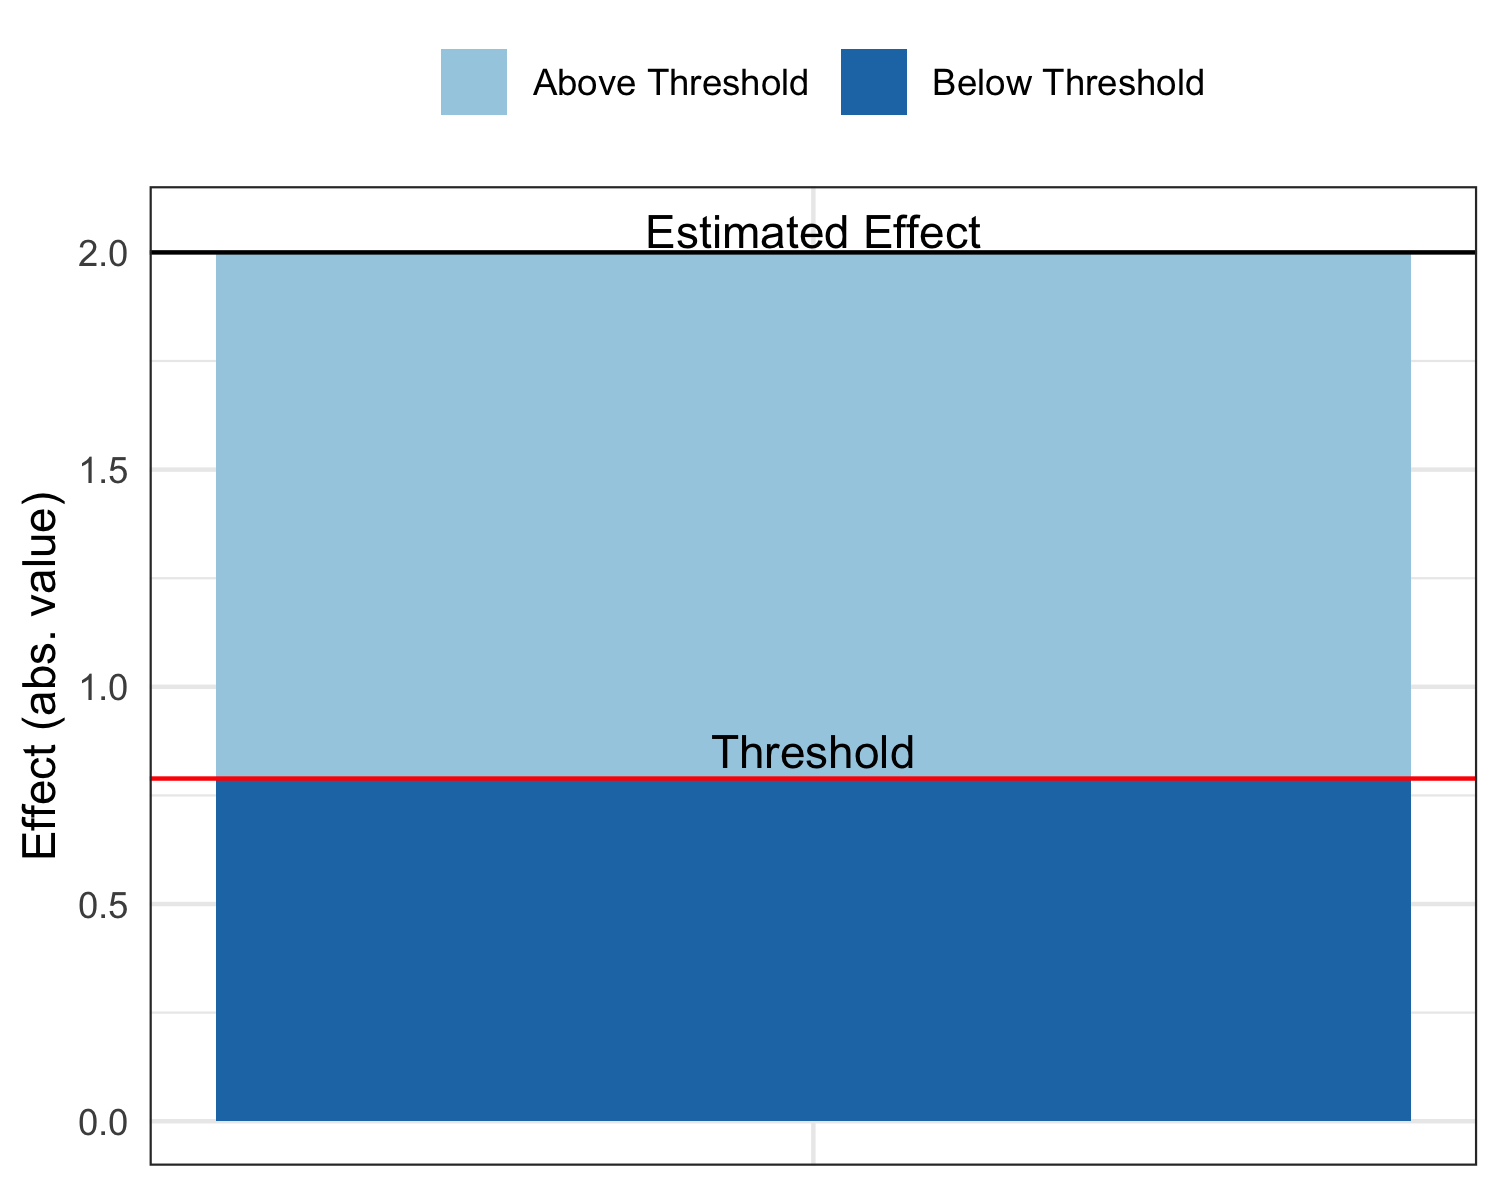
\includegraphics[width=0.7\linewidth]{paper_files/figure-latex/unnamed-chunk-8-1} 

}

\caption{ }\label{fig:unnamed-chunk-81}
\end{figure}\begin{figure}

{\centering 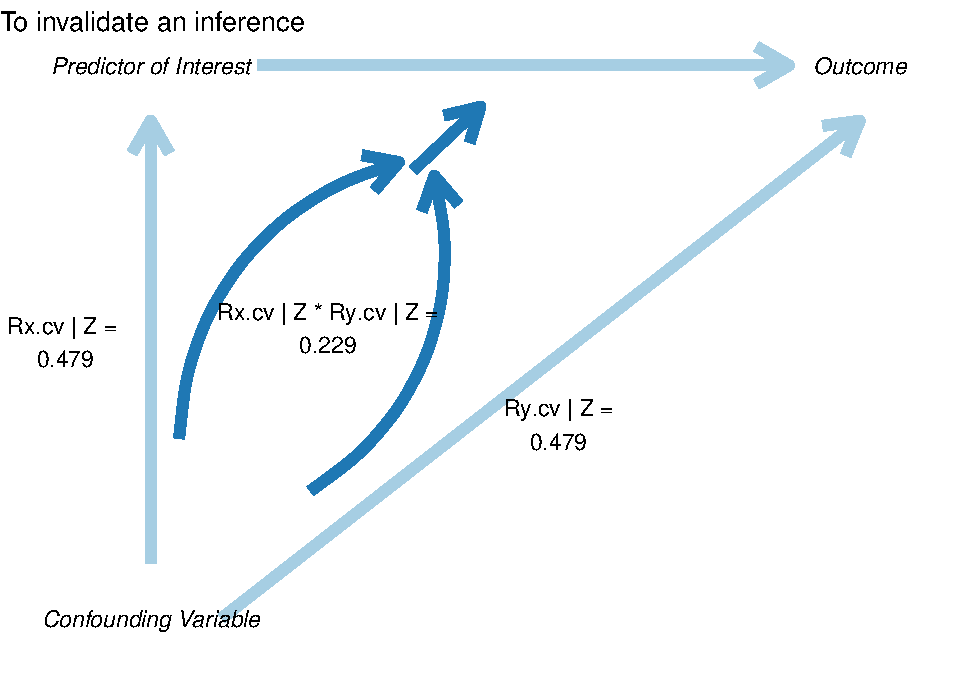
\includegraphics[width=0.7\linewidth]{paper_files/figure-latex/unnamed-chunk-8-2} 

}

\caption{ }\label{fig:unnamed-chunk-82}
\end{figure}

Finally, you can return the raw output, for use in other analyses.

\begin{verbatim}
#> # A tibble: 1 x 8
#>   action inference percent_bias_to~ replace_null_ca~ unstd_beta
#>   <chr>  <chr>                <dbl>            <dbl>      <dbl>
#> 1 to_su~ fail_to_~             89.9               90        0.4
#> # ... with 3 more variables: beta_threshhold <dbl>,
#> #   omitted_variable_corr <dbl>, itcv <dbl>
\end{verbatim}

\subsection{Use of konfound() for models fit in
R}\label{use-of-konfound-for-models-fit-in-r}

Where \texttt{pkonfound()} can be used with values from
already-conducted analyses, \texttt{konfound()} can be used with models
(\texttt{lm()}, \texttt{glm()}, and \texttt{lme4::lmer()}) fit in R.

\subsubsection{Example 2A: For linear models fit with
lm()}\label{example-2a-for-linear-models-fit-with-lm}

\begin{verbatim}
#> 
#> Call:
#> lm(formula = mpg ~ wt + hp + qsec, data = mtcars)
#> 
#> Coefficients:
#> (Intercept)           wt           hp         qsec  
#>    27.61053     -4.35880     -0.01782      0.51083
#> Percent Bias Necessary to Invalidate the Inference:
#> To sustain an inference, 41.327% of the estimate would have to be due to bias. This is based on a threshold of -0.031 for statistical significance (alpha = 0.05).
#> To sustain an inference, 13 of the cases with 0 effect would have to be replaced with cases at the threshold of inference.
#> 
#> Impact Threshold for a Confounding Variable:
#> An omitted variable would have to be correlated at 0.322 with the outcome and at 0.322 with the predictor of interest (conditioning on observed covariates) to sustain an inference based on a threshold of -0.031 for statistical significance (alpha = 0.05).
#> Correspondingly the impact of an omitted variable (as defined in Frank 2000) must be 0.322 X 0.322 = 0.104 to sustain an inference.
\end{verbatim}

Like with \texttt{pkonfound()}, we can also output multiple forms of
output at once with \texttt{konfound()}:

\begin{verbatim}
#> Percent Bias Necessary to Invalidate the Inference:
#> To sustain an inference, 41.327% of the estimate would have to be due to bias. This is based on a threshold of -0.031 for statistical significance (alpha = 0.05).
#> To sustain an inference, 13 of the cases with 0 effect would have to be replaced with cases at the threshold of inference.
#> 
#> Impact Threshold for a Confounding Variable:
#> An omitted variable would have to be correlated at 0.322 with the outcome and at 0.322 with the predictor of interest (conditioning on observed covariates) to sustain an inference based on a threshold of -0.031 for statistical significance (alpha = 0.05).
#> Correspondingly the impact of an omitted variable (as defined in Frank 2000) must be 0.322 X 0.322 = 0.104 to sustain an inference.
#> Created 3 forms of output. To access type: 
#> 
#> konfound_output$raw_output
#> konfound_output$thresh_plot
#> konfound_output$corr_plot
\end{verbatim}

Again, we can type each of those, i.e.:

\begin{verbatim}
#> # A tibble: 1 x 8
#>   action inference percent_bias_to~ replace_null_ca~ unstd_beta
#>   <chr>  <chr>                <dbl>            <dbl>      <dbl>
#> 1 to_su~ fail_to_~             41.3               13     -0.018
#> # ... with 3 more variables: beta_threshhold <dbl>,
#> #   omitted_variable_corr <dbl>, itcv <dbl>
\end{verbatim}

\begin{figure}

{\centering 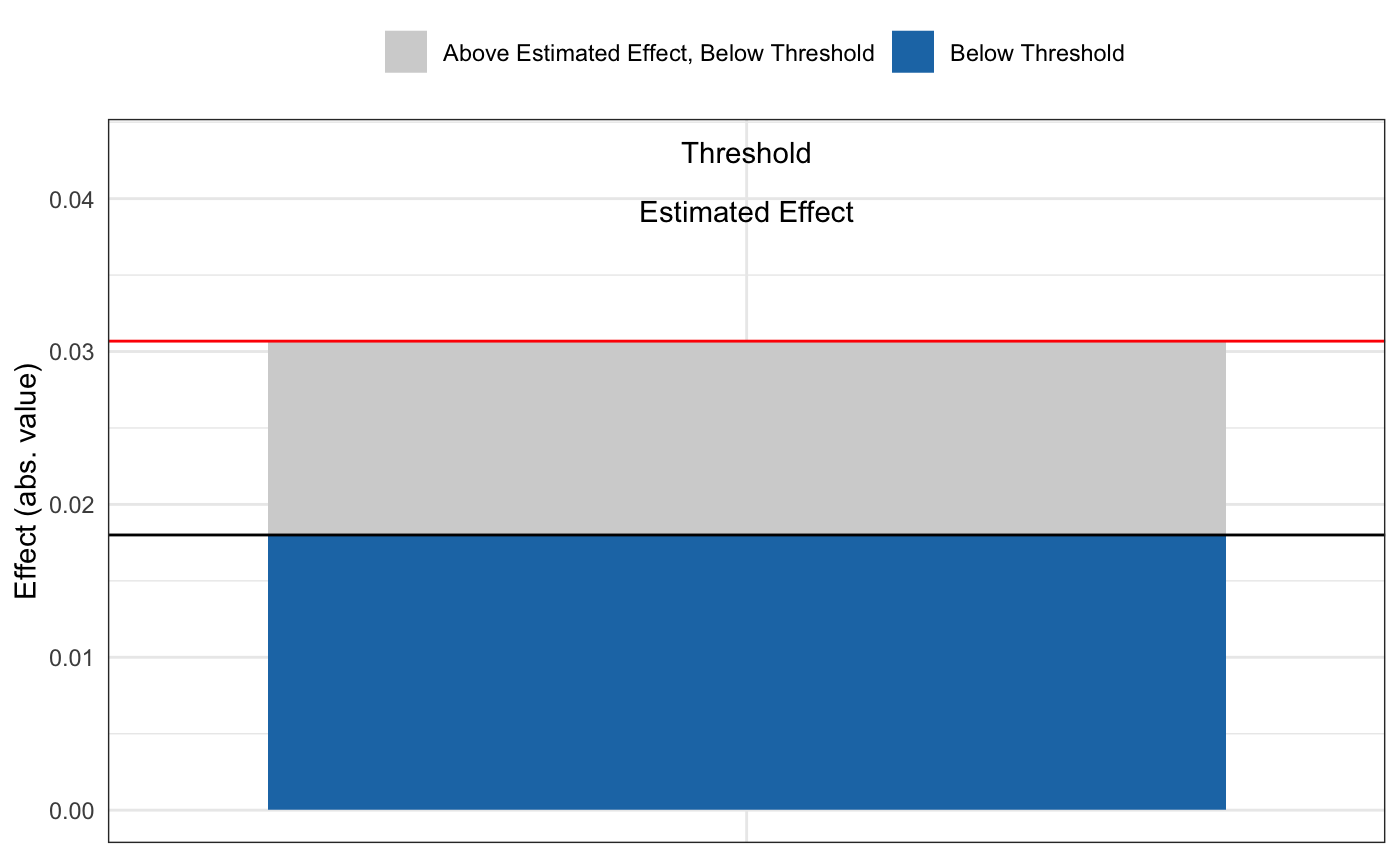
\includegraphics[width=0.7\linewidth]{paper_files/figure-latex/unnamed-chunk-12-1} 

}

\caption{ }\label{fig:unnamed-chunk-12}
\end{figure}

We can also test all of the variables as predictors of interest:

\begin{verbatim}
#> # A tibble: 3 x 8
#>   var_name     t    df action   inference   pct_bias_to_chang~   itcv r_con
#>   <chr>    <dbl> <dbl> <chr>    <chr>                    <dbl>  <dbl> <dbl>
#> 1 wt       -5.79    29 to_inva~ reject_null               51.5  0.585 0.765
#> 2 hp       -1.2     29 to_sust~ fail_to_re~               38.7 -0.102 0.319
#> 3 qsec      1.16    29 to_sust~ fail_to_re~               40.5 -0.106 0.326
\end{verbatim}

Whereas this cannot be carried out with \texttt{pkonfound()}, with
\texttt{konfound()} you can also return a table with some key output
from the correlation-based approach.

\begin{verbatim}
#> Dependent variable is mpg
#> Warning: Unknown or uninitialised column: 'itcv'.
#> Warning: Unknown or uninitialised column: 'impact'.
#> # A tibble: 4 x 7
#>   term        estimate std.error statistic p.value   itcv impact
#>   <chr>          <dbl>     <dbl>     <dbl>   <dbl>  <dbl>  <dbl>
#> 1 (Intercept)   27.6       8.42       3.28   0.003 NA     NA    
#> 2 wt            -4.36      0.753     -5.79   0      0.243 NA    
#> 3 hp            -0.018     0.015     -1.19   0.244 NA      0.511
#> 4 qsec           0.511     0.439      1.16   0.255 NA      0.073
\end{verbatim}

If the impact threshhold is greater than the impacts of the \texttt{Z}s
(the other covariates) then an omitted variable would have to have a
greater impact than any of the observed covariates to change the
inference. Note that in fields in which there is a lot known about
covariates given the outcome of interest, then the omitted ones are
likely less important than those that are known an included (i.e., we
have a good sense of the factors that matter in terms of educational
achievement).

\subsubsection{Example 2B: For generalized linear models fit with
glm()}\label{example-2b-for-generalized-linear-models-fit-with-glm}

Effects for these models are interpreted on the basis of average partial
(or marginal) effects (calculated using the \texttt{margins} package).

\begin{verbatim}
#> Percent Bias Necessary to Invalidate the Inference:
#> To sustain an inference, 80.978% of the estimate would have to be due to bias. This is based on a threshold of 0.013 for statistical significance (alpha = 0.05).
#> To sustain an inference, 17334 of the cases with 0 effect would have to be replaced with cases at the threshold of inference.
#> 
#> Impact Threshold for a Confounding Variable:
#> An omitted variable would have to be correlated at 5.535 with the outcome and at 5.535 with the predictor of interest (conditioning on observed covariates) to invalidate an inference based on a threshold of 1.003 for statistical significance (alpha = 0.05).
#> Correspondingly the impact of an omitted variable (as defined in Frank 2000) must be 5.535 X 5.535 = 30.636 to invalidate an inference.
#> NULL
\end{verbatim}

As with models fit with \texttt{lm()} (and use of \texttt{pkonfound()}),
multiple forms of output can be specified with the \texttt{to\_return}
argument to \texttt{konfound()}, i.e.
\texttt{konfound(m2,\ age,\ to\_return\ =\ c("raw\_output",\ "corr\_plot",\ "thresh\_plot"))}.

\subsubsection{Example 2C: For mixed effects (or multi-level) models fit
with the lmer() function from the lme4
package}\label{example-2c-for-mixed-effects-or-multi-level-models-fit-with-the-lmer-function-from-the-lme4-package}

\texttt{konfound} also works with models fit with the \texttt{lmer()}
function from the package \texttt{lme4}, for mixed-effects or
multi-level models. One challenge with carrying out sensitivity analysis
for fixed effects in mixed effects models is calculating the correct
denominator degrees of freedom for the t-test associated with the
coefficients. This is not unique to sensitivity analysis, as, for
example, \texttt{lmer()} does not report degrees of freedom (or
p-values) for fixed effects predictors (see this information in the
\texttt{lme4} FAQ
\href{http://bbolker.github.io/mixedmodels-misc/glmmFAQ.html\#why-doesnt-lme4-display-denominator-degrees-of-freedomp-values-what-other-options-do-i-have}{here}).
While it may be possible to determine the correct degrees of freedom for
some models (i.e., models with relatively simple random effects
structures), it is difficult to generalize this approach, and so in this
package the Kenward-Roger approximation for the denominator degrees of
freedom as implemented in the \texttt{pbkrtest} package (described in
\href{https://www.jstatsoft.org/htaccess.php?volume=59\&type=i\&issue=09\&paper=true}{Halekoh
and Højsgaard, 2014}).

Here is an example of the use of \texttt{konfound()} with a model fit
with \texttt{lmer()}:

\begin{verbatim}
#> Warning in bind_rows_(x, .id): binding factor and character vector,
#> coercing into character vector
#> Warning in bind_rows_(x, .id): binding character and factor vector,
#> coercing into character vector
#> Percent Bias Necessary to Invalidate the Inference:
#> To invalidate an inference, 84.83% of the estimate would have to be due to bias. This is based on a threshold of 1.588 for statistical significance (alpha = 0.05).
#> To invalidate an inference, 137 observations would have to be replaced with cases for which the effect is 0.
#> 
#> Impact Threshold for a Confounding Variable:
#> An omitted variable would have to be correlated at 0.817 with the outcome and at 0.817 with the predictor of interest (conditioning on observed covariates) to invalidate an inference based on a threshold of 0.155 for statistical significance (alpha = 0.05).
#> Correspondingly the impact of an omitted variable (as defined in Frank 2000) must be 0.817 X 0.817 = 0.667 to invalidate an inference.
#> NULL
\end{verbatim}

\subsubsection{Example 2D: Use of mkonfound() for meta-analyses that
include sensitivity
analysis}\label{example-2d-use-of-mkonfound-for-meta-analyses-that-include-sensitivity-analysis}

We can also use \texttt{konfound} to carry out sensitivity analysis as
part of meta-analyses. For example, here, \texttt{d} represents output
from a number (30 in this case) of past studies, read in a CSV file from
a website:

\begin{verbatim}
#>           t  df
#> 1  7.076763 178
#> 2  4.127893 193
#> 3  1.893137  47
#> 4 -4.166395 138
#> 5 -1.187599  97
#> 6  3.585478  87
#> # A tibble: 30 x 7
#>         t    df action     inference     pct_bias_to_change_i~   itcv r_con
#>     <dbl> <int> <chr>      <chr>                         <dbl>  <dbl> <dbl>
#>  1  7.08    178 to_invali~ reject_null                   68.8   0.378 0.614
#>  2  4.13    193 to_invali~ reject_null                   50.6   0.168 0.41 
#>  3  1.89     47 to_sustain fail_to_reje~                  5.47 -0.012 0.11 
#>  4 -4.17    138 to_invali~ reject_null                   50.3   0.202 0.449
#>  5 -1.19     97 to_sustain fail_to_reje~                 39.4  -0.065 0.255
#>  6  3.59     87 to_invali~ reject_null                   41.9   0.19  0.436
#>  7  0.282   117 to_sustain fail_to_reje~                 85.5  -0.131 0.361
#>  8  2.55     75 to_invali~ reject_null                   20.6   0.075 0.274
#>  9 -4.44    137 to_invali~ reject_null                   53.0   0.225 0.475
#> 10 -2.05    195 to_invali~ reject_null                    3.51  0.006 0.077
#> # ... with 20 more rows
\end{verbatim}

We can also return a plot summarizing the percent bias needed to sustan
or invalidate an inference across all of the past studies:

\begin{figure}

{\centering 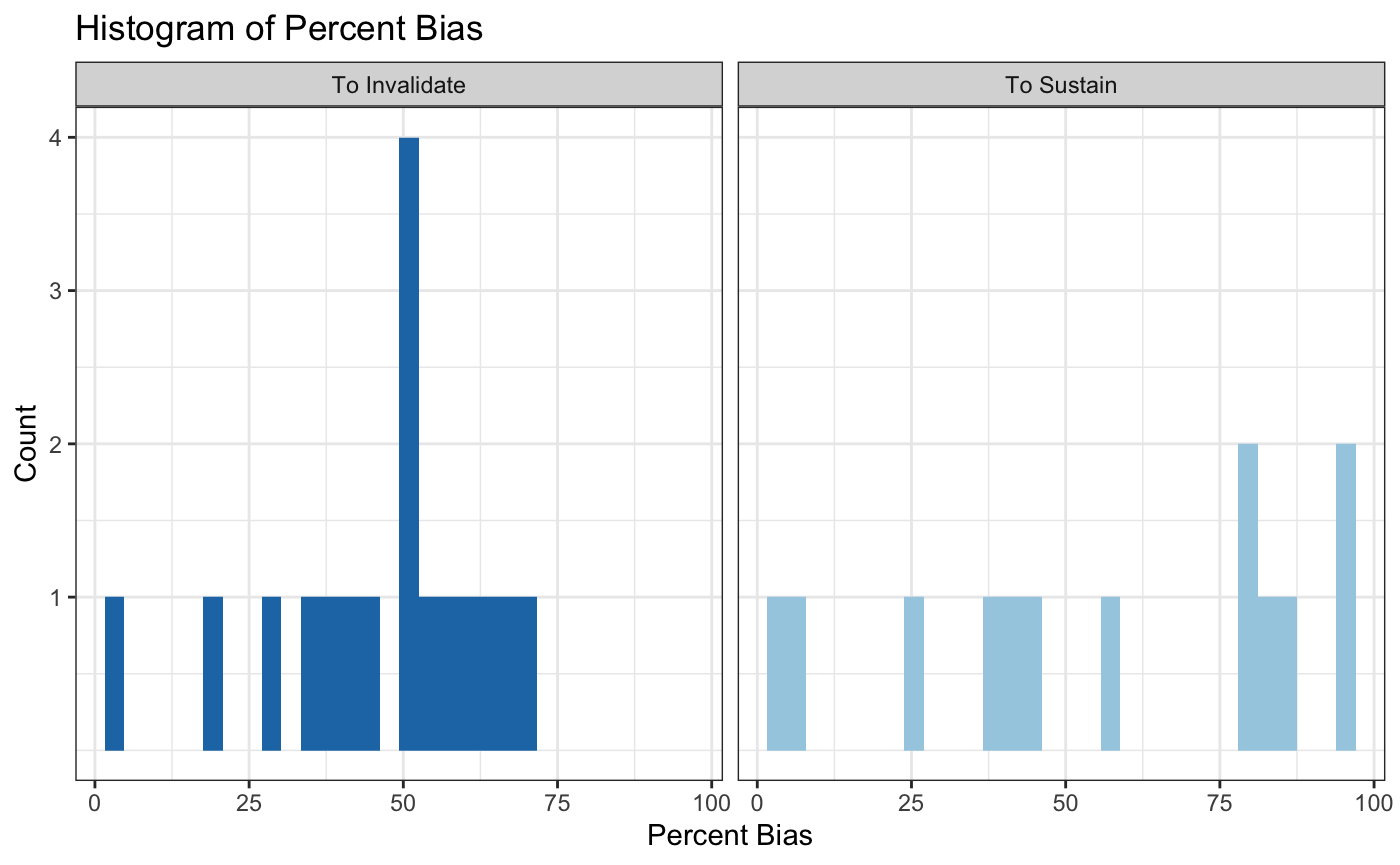
\includegraphics[width=0.7\linewidth]{paper_files/figure-latex/unnamed-chunk-18-1} 

}

\caption{ }\label{fig:unnamed-chunk-18}
\end{figure}

\section{Examples of publishable
write-ups}\label{examples-of-publishable-write-ups}

(from Beymer) (for correlation-based approach) (ref appendix)

\section{References}\label{references}

Behn, R.D. and Vaupel, J.W., 1982. Quick analysis for busy decision
makers (p.~3). New York: Basic Books. Cohen, J., Cohen, P., West, S.G.
and Aiken, L.S., 1983. Applied multiple regression for the behavioral
sciences. Laurence Erlbaum, Hillsdale, NJ. DiPrete, T.A. and Gangl, M.,
2004. Assessing bias in the estimation of causal effects: Rosenbaum
bounds on matching estimators and instrumental variables estimation with
imperfect instruments. Sociological methodology, 34(1), pp.271-310.
Frank, K. A. and Min, K. 2007. Indices of Robustness for Sample
Representation. Sociological Methodology. Vol 37, 349-392. Frank, K.A.
2000. Impact of a Confounding Variable on the Inference of a Regression
Coefficient. Sociological Methods and Research, 29(2), 147-194 Frank,
K.A., Gary Sykes, Dorothea Anagnostopoulos, Marisa Cannata, Linda Chard,
Ann Krause, Raven McCrory. 2008. Extended Influence: National Board
Certified Teachers as Help Providers. Education, Evaluation, and Policy
Analysis. Vol 30(1): 3-3 Frank, K.A., Maroulis, S., Duong, M., and
Kelcey, B. 2013. What would it take to Change an Inference?: Using
Rubin's Causal Model to Interpret the Robustness of Causal Inferences.
Education, Evaluation and Policy Analysis. Vol 35: 437-460. Gill, R.D.
and Robins, J.M., 2001. Causal inference for complex longitudinal data:
the continuous case. Annals of Statistics, pp.1785-1811. Hamilton, L.C.,
1983. Saving water: a causal model of household conservation.
Sociological Perspectives, 26(4), pp.355-374. Hamilton, L.C., 1985.
Concern about toxic wastes: Three demographic predictors. Sociological
Perspectives, 28(4), pp.463-486. Hamilton, L.C., 1992. Regression with
graphics: A second course in applied statistics. Pan, W., and Frank,
K.A. 2004. An Approximation to the Distribution of the Product of Two
Dependent Correlation Coefficients. Journal of Statistical Computation
and Simulation, 74, 419-443 Pan, W., and Frank, K.A., 2004. A
probability index of the robustness of a causal inference. Journal of
Educational and Behavioral Statistics, 28, 315-337. Robins, J. 1987.
\enquote{A Graphical Approach to the Identification and Estimation of
Causal Parameters inMortality Studies with Sustained Exposure Periods.}
Journal of Chronic Diseases 40(2):1395--1615. Robins, J., A. Rotnisky,
and D. Scharfstein. 2000. \enquote{Sensitivity Analysis for Selection
Bias and Unmeasured Confounding in Missing Data and Causal Inference
Models.} Pp. 1--95 in Statistical Models in Epidemiology,the Environment
and Clinical Trials (The IMA Volumes in Mathematics and Its
Applications), edited by E. Halloran and D. Berry. New York:
Springer-Verlag. Rosenbaum, P. R. 1986. \enquote{Dropping Out of High
School in the United States: An Observational Study.} Journal of
Educational Statistics 11(3):207--24. Rosembaum, P. R. 2002.
\enquote{AttributionEffects to Treatment inMatched Observational
Studies.} Journal of the American Statistical Association 97:183--92.
Rubin, D. B. 1974. \enquote{Estimating Causal Effects of Treatments in
Randomized and Nonrandomized Studies.} Journal of Educational Psychology
66:688--701. Saw, G., Schneider, B., Frank, K., Chen, I.C., Keesler, V.
and Martineau, J., 2017. The Impact of Being Labeled as a Persistently
Lowest Achieving School: Regression Discontinuity Evidence on
Consequential School Labeling. American Journal of Education, 123(4),
pp.585-613. Scharfstein, D. A. I. 2002. \enquote{Generalized Additive
Selection Models for the Analysis of Studies with Potentially
Nonignorable Missing Data.} Biometrics 59:601--13. VanderWeele, T.J. and
Arah, O.A., 2011. Bias formulas for sensitivity analysis of unmeasured
confounding for general outcomes, treatments, and confounders.
Epidemiology (Cambridge, Mass.), 22(1), pp.42-52. VanderWeele, T.J.,
2010. Bias formulas for sensitivity analysis for direct and indirect
effects. Epidemiology (Cambridge, Mass.), 21(4), p.540. Wooldridge,
J.M., 2010. Econometric analysis of cross section and panel data. MIT
press.


\end{document}
